\documentclass{article}
\usepackage{amsmath,amssymb,graphicx,hyperref}

\title{Speeding Up Matrix Multiplication with Machine Learning}
\author{Manan Bhatia}
\date{\today}

\begin{document}

\maketitle

\section{Introduction}
Matrix multiplication is a fundamental operation required in various fields, including machine learning, computer science, computer graphics, and scientific simulations. The standard matrix multiplication algorithm executes in cubic time complexity, \( O(N^3) \), making it a computational bottleneck for large-scale systems such as neural networks and transformer architectures.

More efficient algorithms, such as Strassen’s and the Coppersmith-Winograd algorithm, demonstrate that faster approaches are possible. However, the search for continuously faster algorithms has mostly been manual, constrained by human intuition and the vast combinatorial nature of the problem space. 

Through research presented in \textit{“Discovering Faster Matrix Multiplication”}, we learn that reinforcement learning extends previous work by accelerating the mathematical exploration of matrix multiplication. The AlphaZero-inspired AlphaTensor agent discovers optimal tensor decompositions in finite factor spaces, rediscovering known algorithms and discovering new ones that outperform traditional methods for smaller matrix sizes.

\begin{figure}[h]
    \centering
    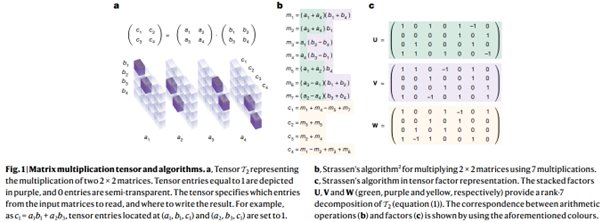
\includegraphics[width=0.8\linewidth]{Picture1.png}
    \caption{Tensor representation of matrix multiplication as a rank-3 tensor. Lower-rank decompositions reduce scalar multiplications. (Source: AlphaTensor paper)}
    \label{fig:tensor-representation}
\end{figure}

This research expands on previous work by studying matrix multiplication mathematics while implementing reinforcement learning models inspired by AlphaZero to evaluate performance and explore new optimization techniques.

\section{Literature Review}


\end{document}